\documentclass[12pt]{article}

% ----------- PACKAGES -----------
\usepackage[utf8]{inputenc}
\usepackage{graphicx}
\usepackage{amsmath}
\usepackage{amssymb}
\usepackage{float}
\usepackage{hyperref}
\usepackage{caption}
\usepackage{booktabs}
\usepackage{tikz}
\usepackage{enumitem}
\usepackage{titlesec}
\usepackage{svg}
% \usepackage{cite}
\usepackage[margin=1in]{geometry}
\usepackage{siunitx}
\usepackage{pgfplots}
\usepackage{pdfpages}
\usepackage{subcaption}

% ----------- FORMATTING -----------
\setlength{\parskip}{0.5em}
\setlength{\parindent}{0pt}
\captionsetup{font=small}
\renewcommand{\figurename}{Figure}
\renewcommand{\tablename}{Table}


% ----------- TITLE -----------
\title{ECSE-4320 Project 3 \\ \large SSD Performance Profiling}
\author{Timon Cappella-Pimor}
\date{\today}

% ==================================
\begin{document}
% \pagenumbering{gobble}
\maketitle
\newpage
\section*{Methodology}

All experiments run using fio on a 256 GiB file on an EXT-4 filesystem.


Linux Kernel Version: 7.2.11-zen1-1-zen \\
CPU: AMD Ryzen 7 9700X \\
SSD: Samsung 990 Pro 2 TB NVME \\
FIO Version: 3.43 \\
IO engine: io\_uring

\newpage
\section*{Zero-queue Baselines}

\begin{figure}[H]
    \makebox[\textwidth][c]{%
        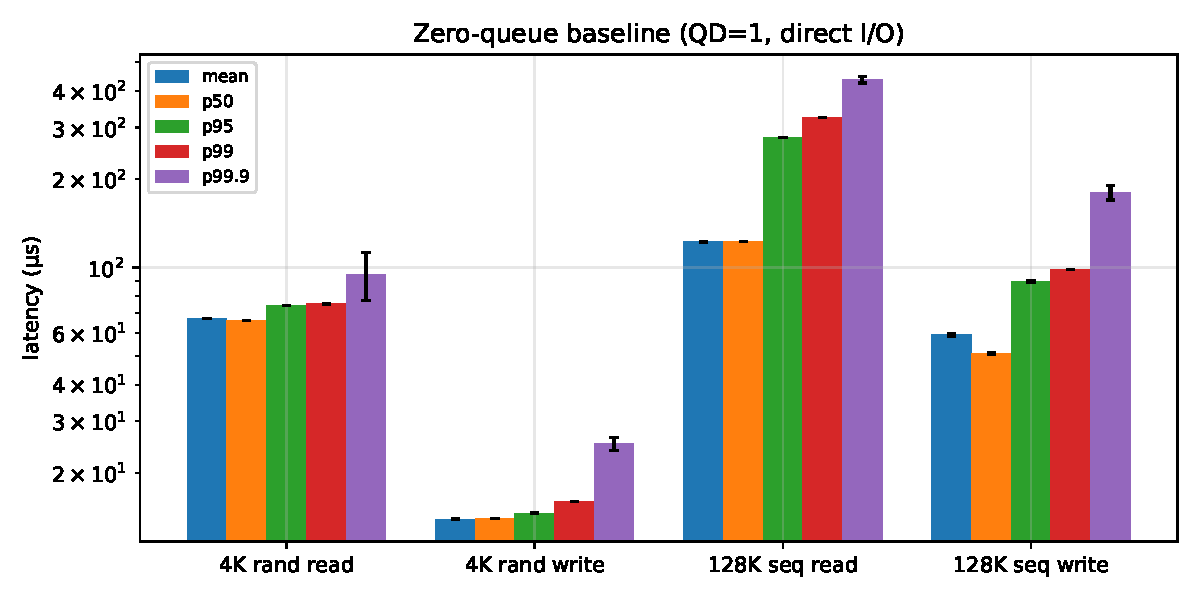
\includegraphics[width=\linewidth]{../results/plots/baseline_latency.pdf}%
    }
    \caption{}
    \label{fig:baseline-latency}
\end{figure}

\newpage
\section*{Block-size and Pattern Sweeps}

\begin{figure}[H]
    \makebox[\textwidth][c]{%
        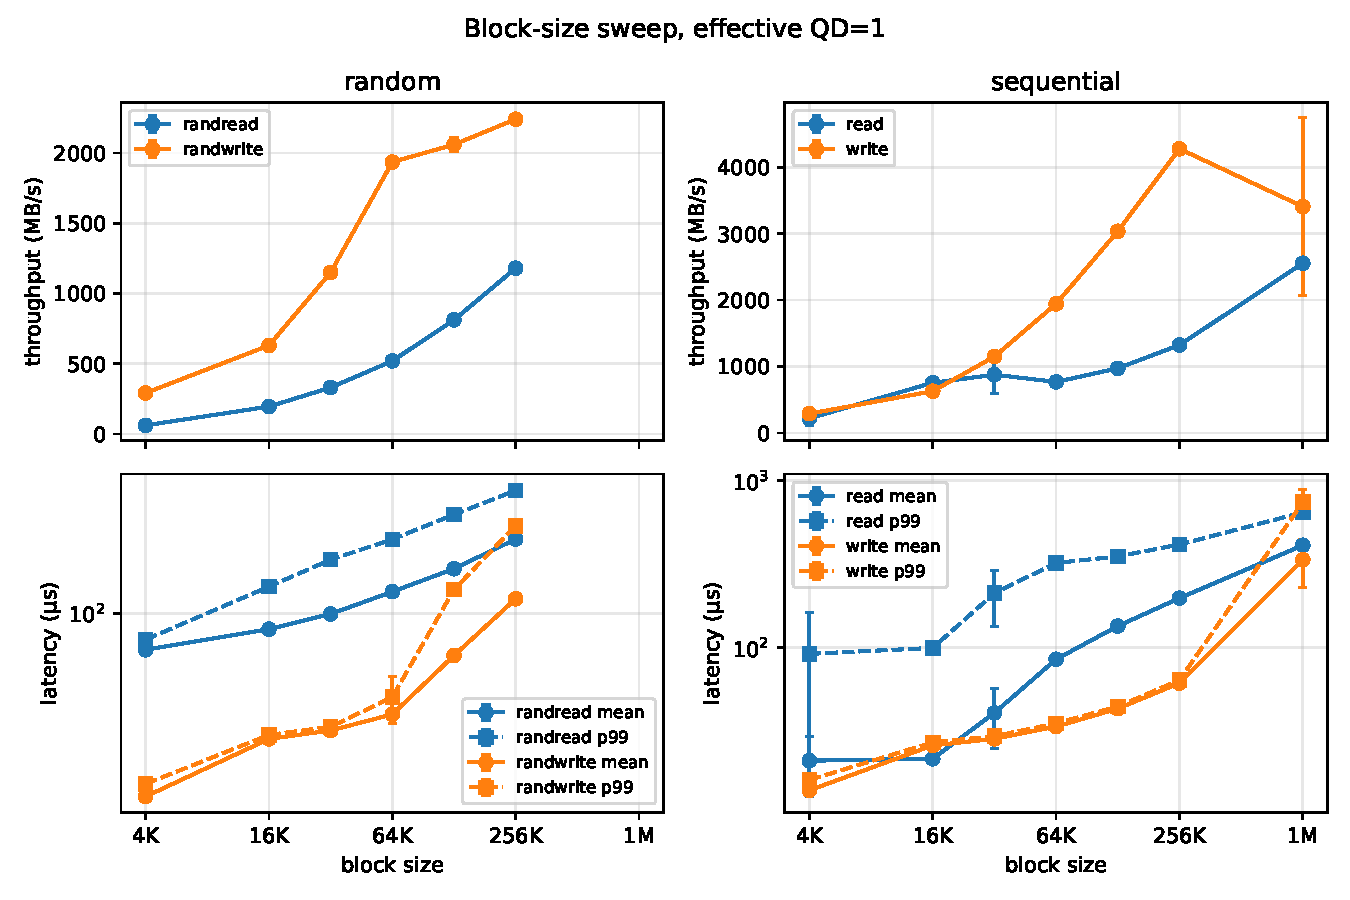
\includegraphics[width=\linewidth]{../results/plots/blocksize_qd1.pdf}%
    }
    \caption{}
    \label{fig:blocksize-qd1}
\end{figure}

\begin{figure}[H]
    \makebox[\textwidth][c]{%
        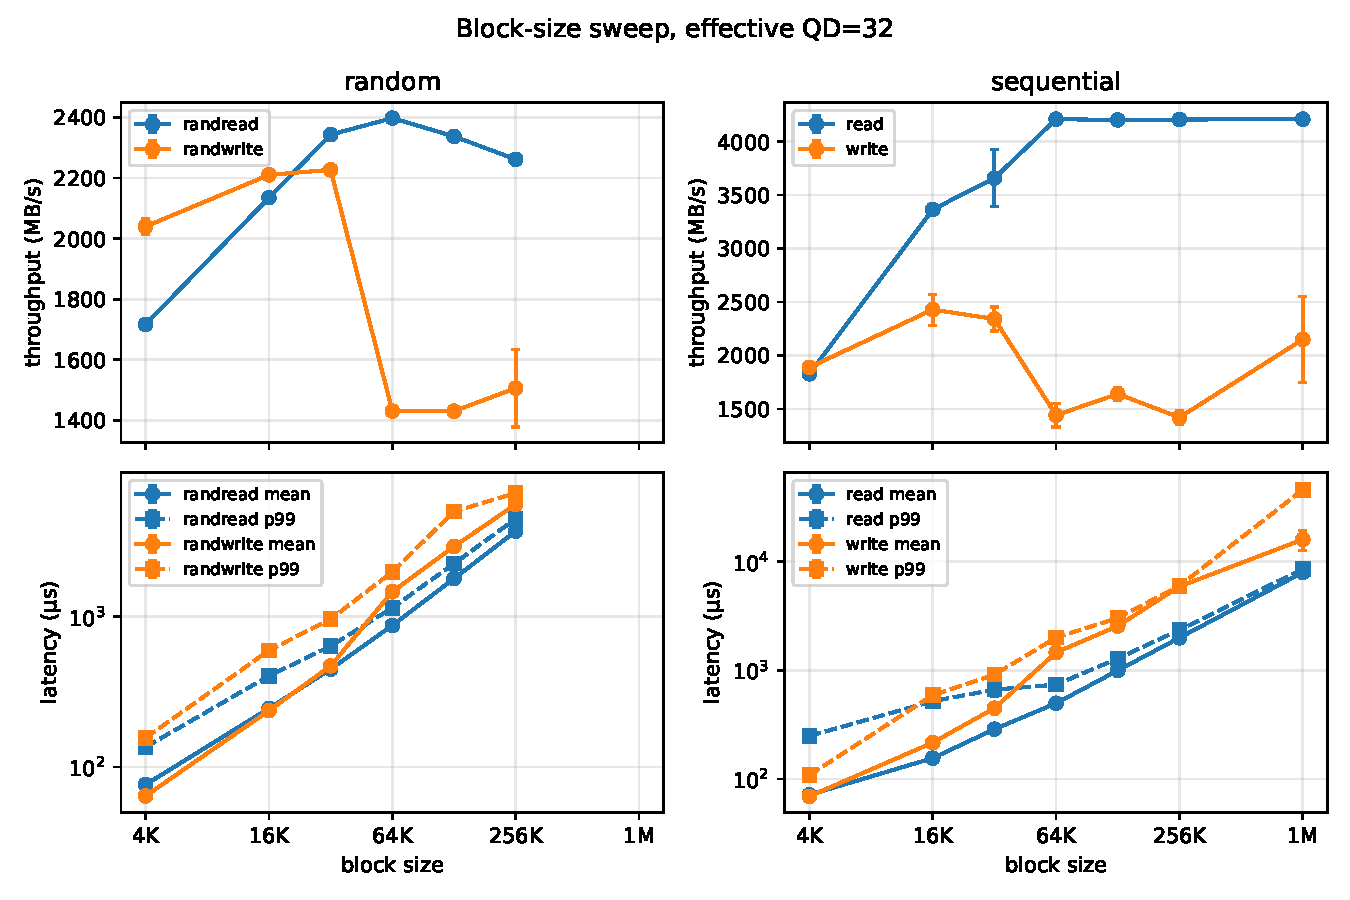
\includegraphics[width=\linewidth]{../results/plots/blocksize_qd32.pdf}%
    }
    \caption{}
    \label{fig:blocksize-qd32}
\end{figure}

\begin{figure}[H]
    \makebox[\textwidth][c]{%
        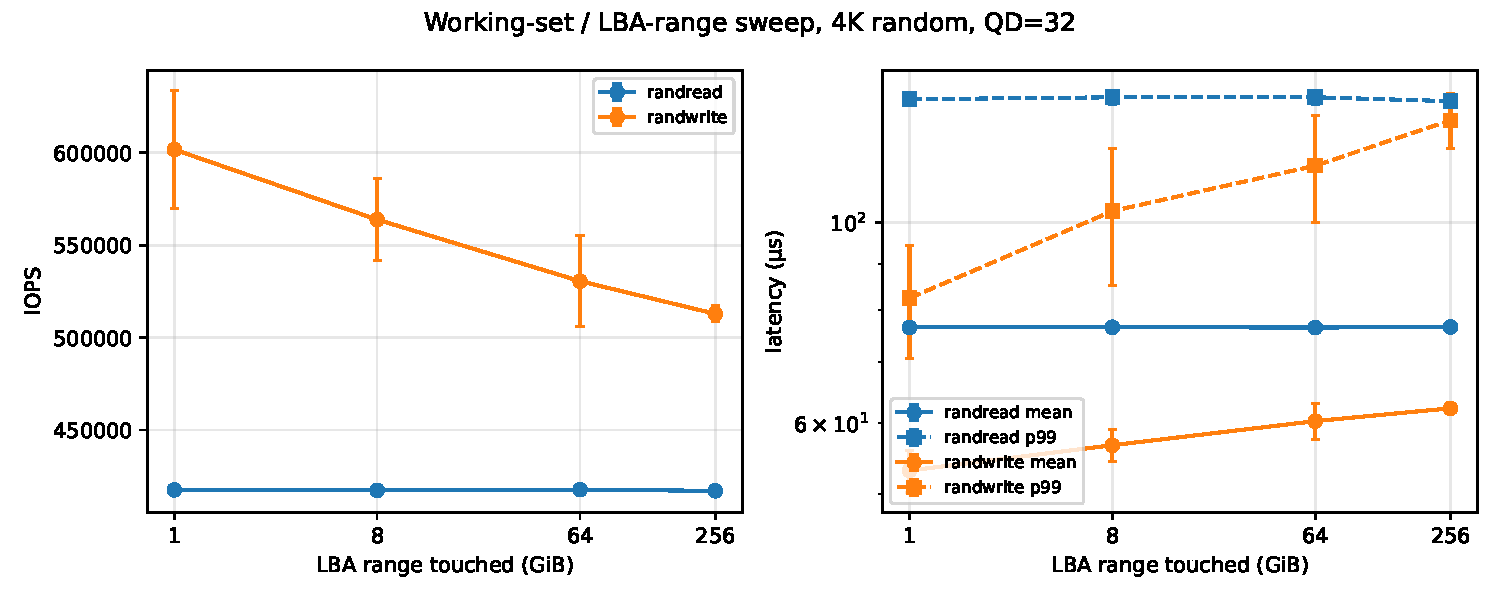
\includegraphics[width=\linewidth]{../results/plots/range.pdf}%
    }
    \caption{}
    \label{fig:range}
\end{figure}

\newpage
\section*{Read/Write and Queue-depth Analysis}

\begin{figure}[H]
    \makebox[\textwidth][c]{%
        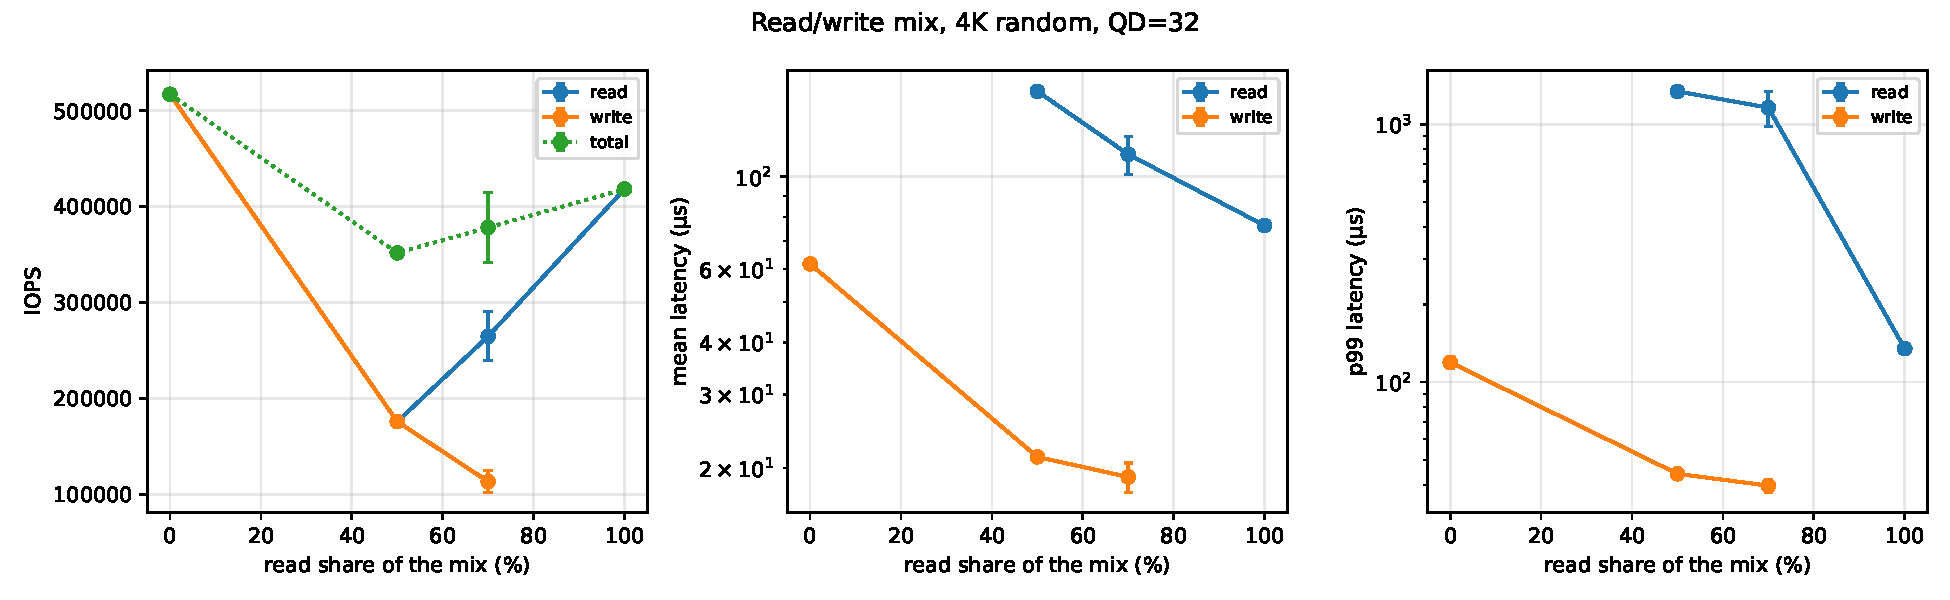
\includegraphics[width=\linewidth]{../results/plots/rwmix.pdf}%
    }
    \caption{}
    \label{fig:rwmix}
\end{figure}

\begin{figure}[H]
    \makebox[\textwidth][c]{%
        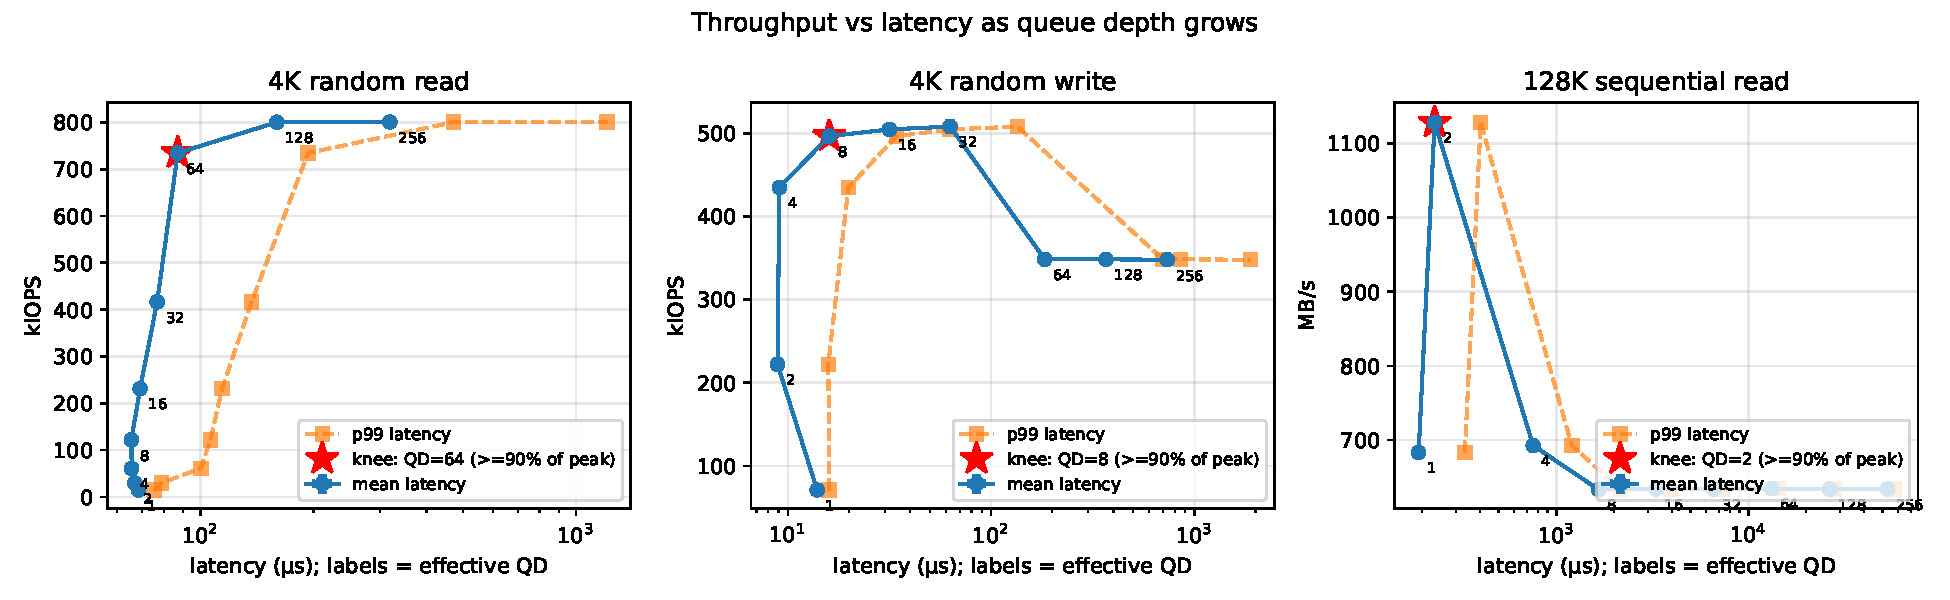
\includegraphics[width=\linewidth]{../results/plots/qd_curve.pdf}%
    }
    \caption{}
    \label{fig:qd-curve}
\end{figure}

\begin{figure}[H]
    \makebox[\textwidth][c]{%
        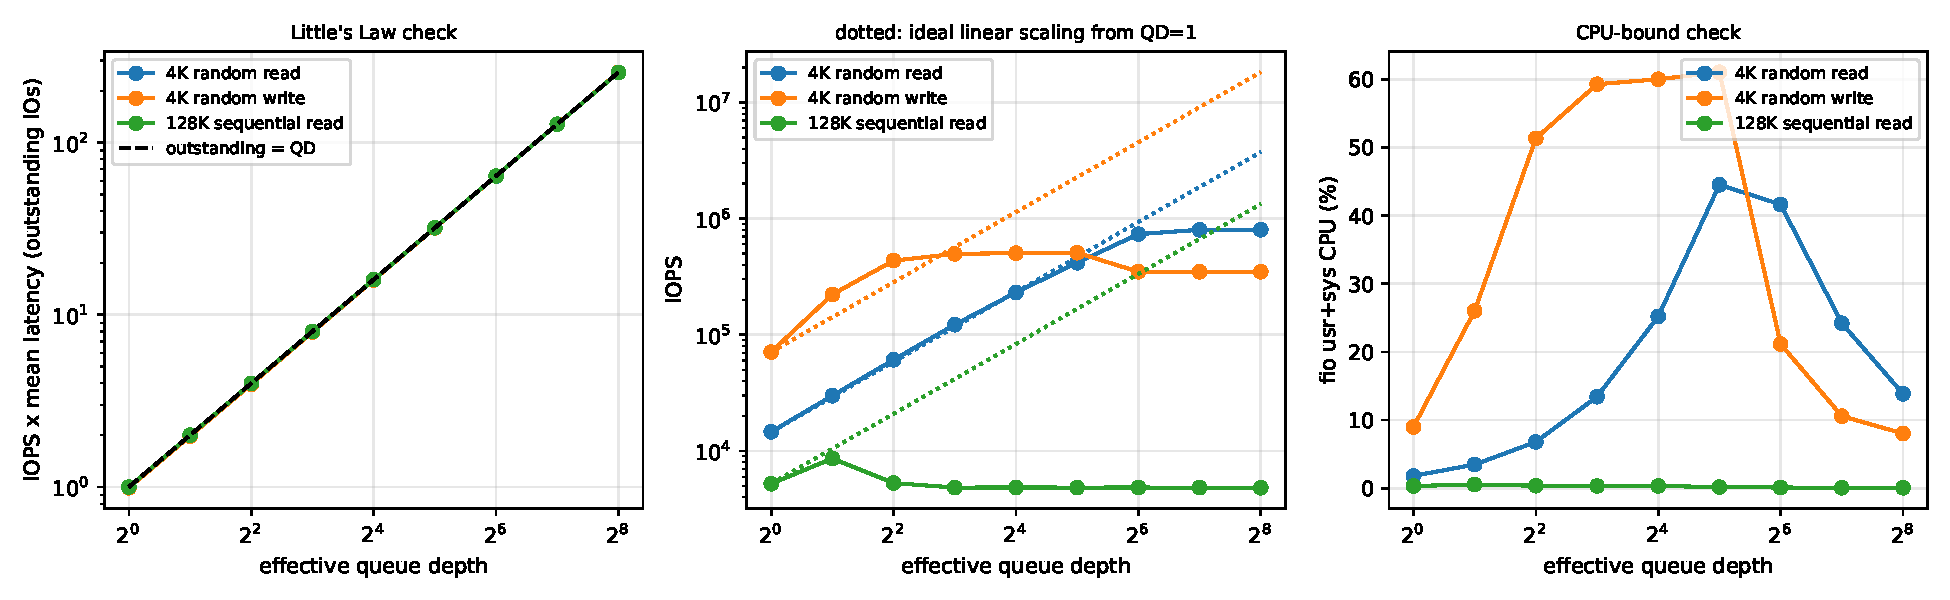
\includegraphics[width=\linewidth]{../results/plots/qd_littles_law.pdf}%
    }
    \caption{}
    \label{fig:qd-littles-law}
\end{figure}


\newpage
\section*{Tail Latency and Device State}

\begin{figure}[H]
    \makebox[\textwidth][c]{%
        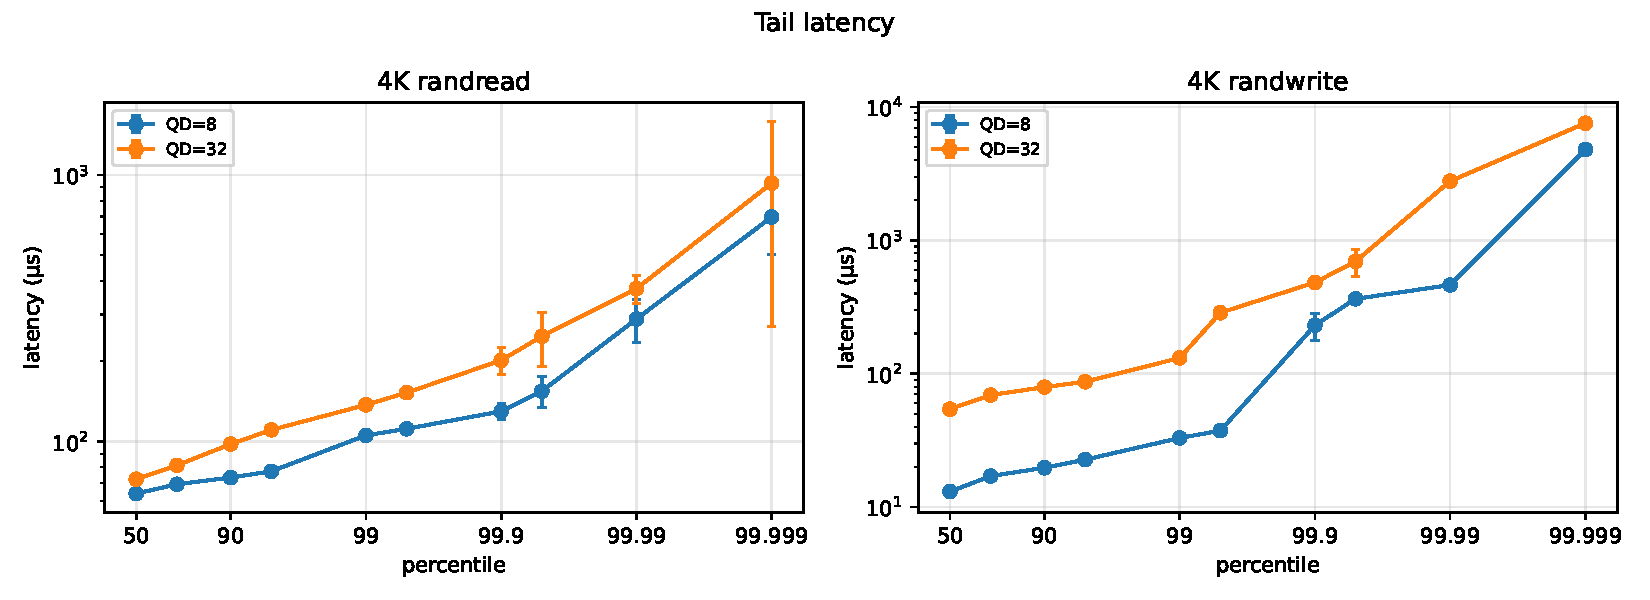
\includegraphics[width=\linewidth]{../results/plots/tail.pdf}%
    }
    \caption{}
    \label{fig:tail}
\end{figure}

\begin{figure}[H]
    \makebox[\textwidth][c]{%
        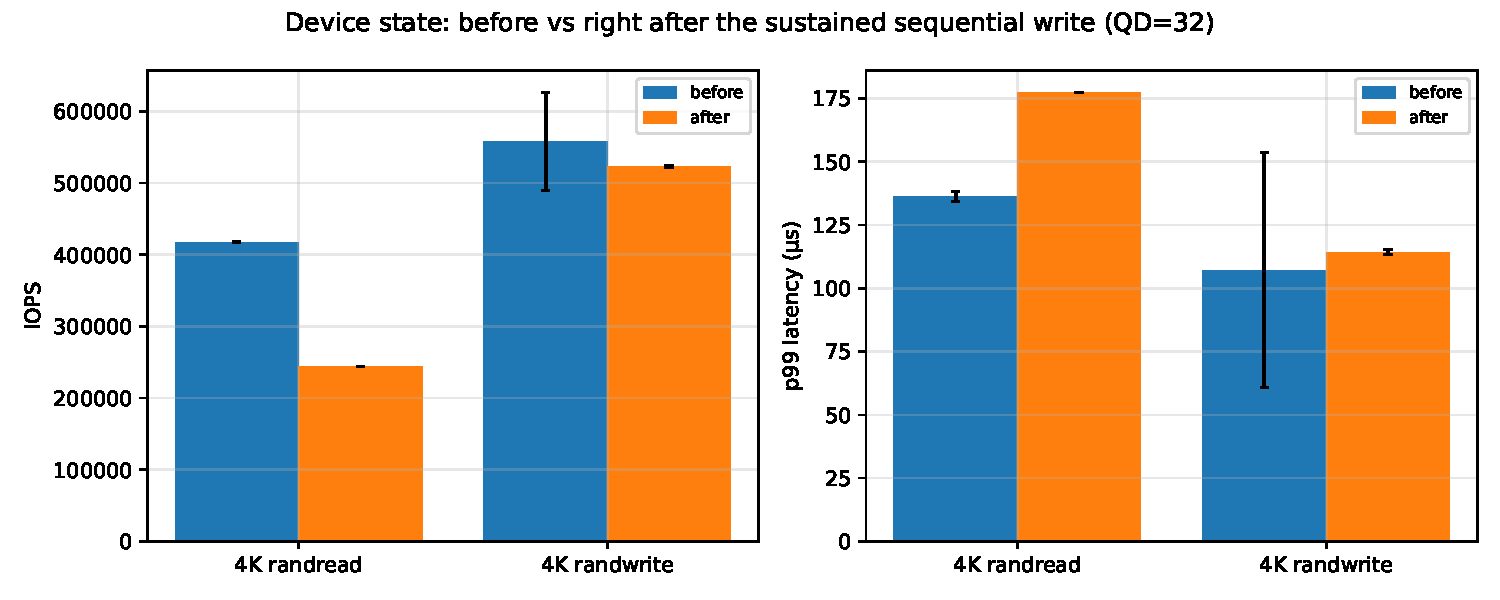
\includegraphics[width=\linewidth]{../results/plots/state_compare.pdf}%
    }
    \caption{}
    \label{fig:state-compare}
\end{figure}

\begin{figure}[H]
    \makebox[\textwidth][c]{%
        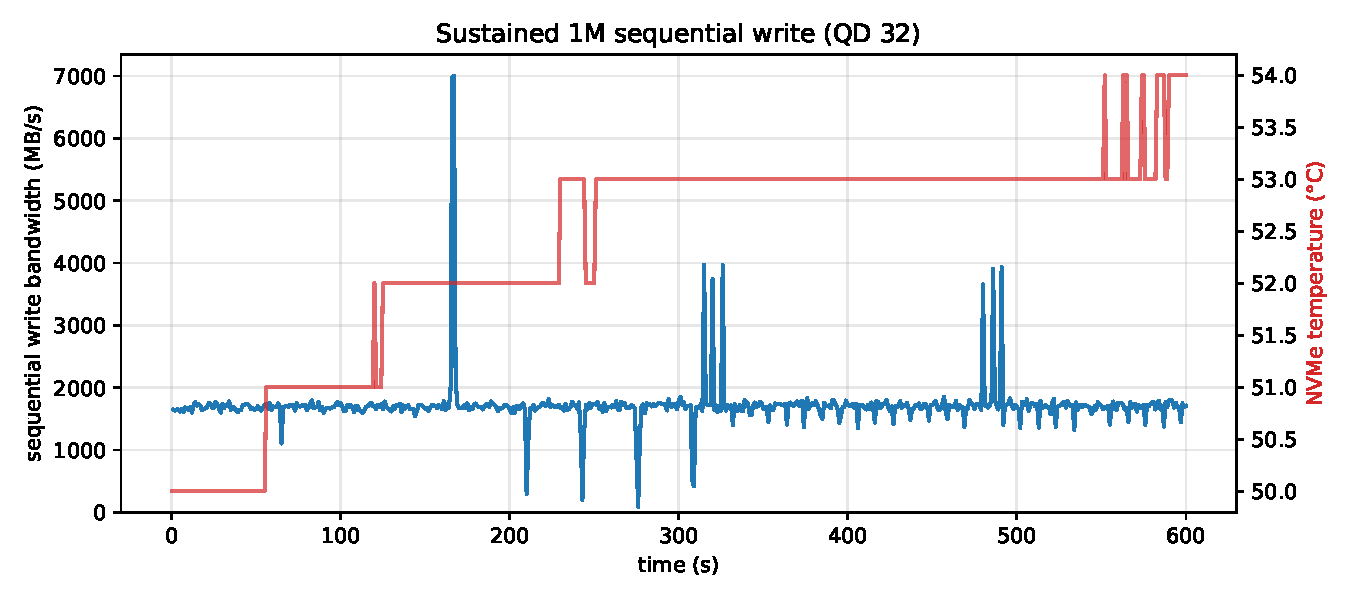
\includegraphics[width=\linewidth]{../results/plots/state_timeseries.pdf}%
    }
    \caption{}
    \label{fig:state-timeseries}
\end{figure}


\newpage
\section*{Pitfall Analysis}

\begin{figure}[H]
    \makebox[\textwidth][c]{%
        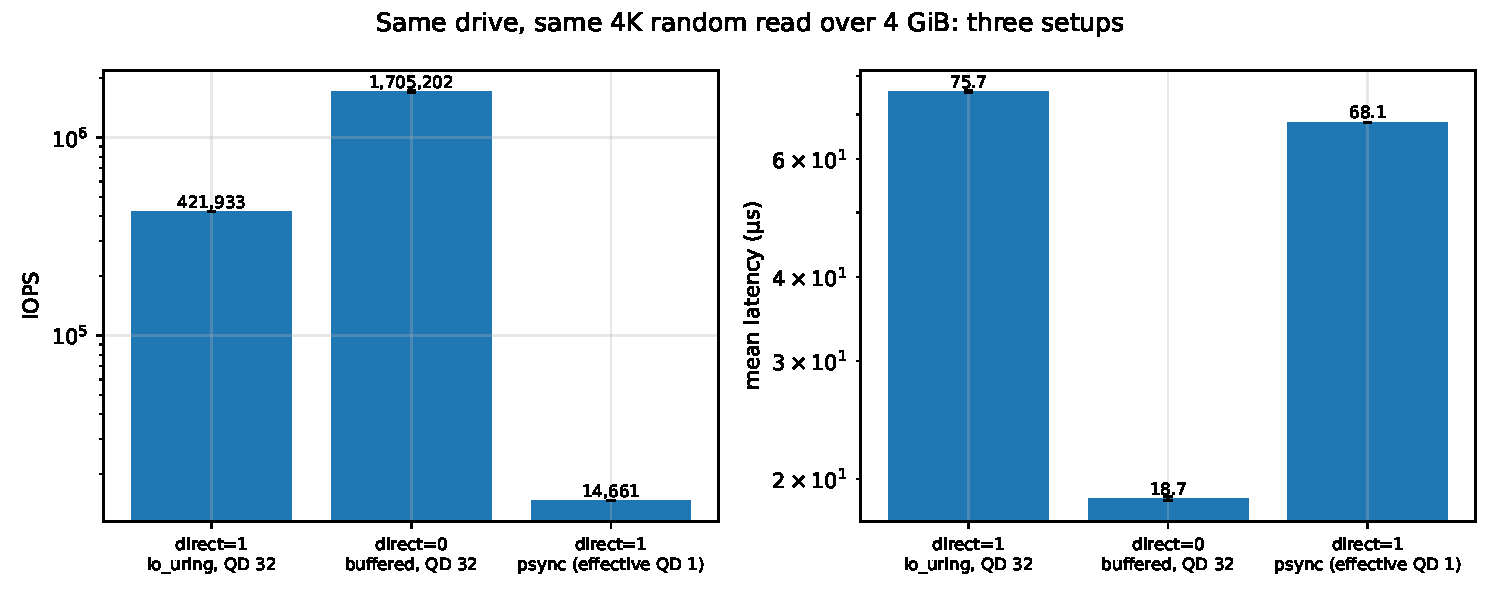
\includegraphics[width=\linewidth]{../results/plots/pitfall.pdf}%
    }
    \caption{}
    \label{fig:pitfall}
\end{figure}

\newpage
\section*{AI-use Transparency}

Claude Sonnet 5.5 was used to write all of the benchmark code (shell scripts +
FIO jobs) and Python plotting code. All words in this report are entirely my
own.


% ---- References ----
% \newpage
% \bibliographystyle{IEEEtran}
% \bibliography{references}

\end{document}
